\documentclass[11pt,a4paper]{article}
\usepackage[margin=2.4cm]{geometry}
\usepackage[T1]{fontenc}
\usepackage{lmodern}
\usepackage{amsmath,amssymb}
\usepackage{booktabs}
\usepackage{multirow}
\usepackage{float}
\usepackage{graphicx}
\usepackage{siunitx}
\usepackage{microtype}
\usepackage{xcolor}
\usepackage{pgfplots}
\pgfplotsset{compat=1.18}
\usepackage[hidelinks]{hyperref}
\sisetup{group-separator={,},group-minimum-digits=4}
\newcommand{\cfg}[1]{\texttt{#1}}
\setlength{\parskip}{0.3em}
\setlength{\emergencystretch}{2em}
\definecolor{s1}{HTML}{2a78d6}
\definecolor{s2}{HTML}{eb6834}
\definecolor{s3}{HTML}{1baf7a}
\definecolor{inkmuted}{HTML}{6b6a64}

\begin{document}

\begin{center}
  {\LARGE Lightweight marine debris detection in\\[0.2em]
  forward-looking sonar on a Raspberry Pi}\\[0.6em]
  {\large Laboratory report, project \texttt{sonar\_edge} (milestones M0--M7)}\\[0.3em]
  15 November 2026
\end{center}
\vspace{0.3em}

\begin{abstract}
\noindent
A one-stage object detector was trained to find and classify ten kinds of
debris (and the tank walls) in whole forward-looking sonar frames, quantised
to 8-bit integers, and executed by a dependency-free C runtime on a
Raspberry Pi~4. The 1\,868 frames of the public water-tank dataset were
grouped into 191 scenes so that near-identical frames never fall on both
sides of a split, and all accuracy figures are pooled five-fold scene
cross-validation. The deployed network (\cfg{small}, $360 \times 240$
input, \num{42463} parameters, 78~M multiply--accumulates) reaches
52.3 $\pm$ 1.7 mAP@0.5 measured on the Pi over three training seeds, and a
2.6 times costlier variant (\cfg{small\_wide}) 56.7 $\pm$ 2.7. The C
runtime is bit-exact with the Python integer reference on every platform.
A hand-written NEON kernel brings the deployed model to 20.3~ms per frame
on one Cortex-A72 core (49 frames/s; 187 frames/s with four independent
copies) in 2.3~MB of memory. Retrained under the same scene folds, the MCNN
crop classifier of the literature falls from 99.8\,\% to 77.7\,\% accuracy;
on its own task, without being given the object boxes, \cfg{small\_wide}
matches it (77.6\,\%) with 20 times fewer parameters, and the deployed
detector processes a frame 4.5 times faster than MCNN classifies the objects
in it.
\end{abstract}

\tableofcontents
\newpage

% ===========================================================================
\section{Aim and objectives}

\textbf{Aim.} To build and measure an end-to-end, embedded-capable system
that detects marine debris in raw forward-looking sonar (FLS) frames, and
to test, under an evaluation protocol free of near-duplicate leakage, the
claim of the MCNN paper \cite{cimen} that its crop classifier is suited to
embedded use.

\textbf{Objectives.}
\begin{enumerate}
  \item Establish a split of the dataset in which test frames are
        independent of training frames (M0).
  \item Design a detector that operates on whole frames and uses only
        operations a minimal integer runtime can execute; choose its size by
        cross-validated accuracy against compute (M1).
  \item Quantise it to 8-bit integers without measurable loss (M2).
  \item Implement a C11 runtime, standard library only, that reproduces the
        integer model bit for bit, and verify it (M3, M4).
  \item Measure latency, throughput, memory and temperature on a
        Raspberry Pi~4, and accelerate the runtime with the processor's
        vector unit without changing its output (M5).
  \item Add a per-pixel segmentation output at negligible cost (M6).
  \item Compare with MCNN under identical data, folds and hardware, for
        accuracy and speed, and measure the deployed system's accuracy on the
        device itself (M7).
\end{enumerate}

% ===========================================================================
\section{Background}

\subsection{Forward-looking sonar}

An FLS such as the ARIS Explorer~3000 emits a fan of acoustic beams and
records the echo intensity along each beam as a function of range. The raw
data are therefore polar (beam angle $\times$ range); for display and for
this dataset they are projected into a Cartesian, fan-shaped image. Objects
appear as bright returns with acoustic shadows behind them, on a dark,
speckled background. Resolution falls with range, and the appearance of an
object depends strongly on viewpoint.

\subsection{MCNN and the predecessor study}

MCNN \cite{cimen} is a convolutional classifier for FLS object crops: the
crop is zero-padded to $305 \times 305$ pixels and passed through six
convolutions and two fully connected layers (2.8~M parameters, 234.7~M
multiply--accumulates per crop) to one of ten classes. It reports 99.87\,\%
accuracy on a random 90/10 split of the \texttt{watertank-cropped} patches
\cite{valdenegro2025}. It does not localise objects: the crops come from
manual annotations.

The predecessor project, \texttt{sonar\_cnn}, reimplemented MCNN and
reproduced the 99.8\,\%, but found two leaks in the protocol
(Table~\ref{tab:predecessor}). First, the crop size alone predicts the
class: a random forest on crop height and width reaches 98.2\,\%. Second,
consecutive sonar frames are near-copies, and a random split places them on
both sides: a nearest-neighbour lookup on $32 \times 32$ thumbnails reaches
100\,\%, and 71\,\% of test crops have a training crop with correlation
above 0.9. On a split that keeps chains of similar crops together, MCNN
drops to 96.6\,\%.

\begin{table}[H]
\centering
\caption{Predecessor study (\texttt{sonar\_cnn}), \texttt{watertank-cropped},
accuracy in \%, mean $\pm$ s.d.\ over 3 seeds.}
\label{tab:predecessor}
\begin{tabular}{lcc}
\toprule
Classifier & Random 80/20 split & Group split \\
\midrule
Random forest on crop $(h, w)$ only & $98.17 \pm 0.70$ & -- \\
1-nearest neighbour, $32 \times 32$ thumbnails & 100.00 & 92.0 \\
MCNN, padded input (paper's setup) & $99.79 \pm 0.17$ & $96.61 \pm 1.98$ \\
MCNN, silhouette only (no image content) & $98.24 \pm 0.55$ & -- \\
\bottomrule
\end{tabular}
\end{table}

\subsection{One-stage, anchor-free detection}

CenterNet \cite{zhou2019} represents each object by its centre point. The
network outputs, on a coarse grid, one heatmap per class whose peaks mark
object centres, plus the box size and a sub-cell offset at each cell.
Decoding needs only a local-maximum test, with no anchor boxes and no
non-maximum suppression, which suits a small integer runtime.

\subsection{Integer quantisation}

In the scheme of Jacob et al.\ \cite{jacob2018}, weights and activations are
stored as 8-bit integers with real-valued scales, products are summed in
32-bit integers, and each layer's result is rescaled to 8 bits by an integer
multiply and shift. Inference then needs no floating-point arithmetic, and
an integer implementation can be made exactly reproducible across
processors.

% ===========================================================================
\section{Materials}

\subsection{Data}

The \texttt{watertank-segmentation} set of the marine debris FLS collection
\cite{valdenegro2025} (repository commit \texttt{4a77998}): 1\,868 frames
from an ARIS Explorer~3000 in a water tank, already projected to Cartesian
coordinates at $320 \times 480$ pixels (width $\times$ height), 8-bit
grey, with 3\,882 bounding boxes in eleven classes
(Table~\ref{tab:classes}); every frame has one to five boxes (mean 2.08).
\emph{Wall} marks the tank walls; it is kept as a class because a deployed
system must not report walls as debris. Pixel-level semantic masks exist for
every frame and are used only by the segmentation head (M6).

\begin{table}[H]
\centering
\caption{Classes and box counts. ``Largest scene'': share of the class's
boxes in the single scene holding most of them, given where it exceeds
40\,\% (Section~\ref{sec:scenes}).}
\label{tab:classes}
\begin{tabular}{lrr@{\hspace{2.5em}}lrr}
\toprule
Class & Boxes & Largest scene & Class & Boxes & Largest scene \\
\midrule
Bottle & 468 & 43\,\% & Shampoo-bottle & 111 & -- \\
Can & 292 & -- & Standing-bottle & 65 & 94\,\% \\
Chain & 320 & -- & Tire & 615 & -- \\
Drink-carton & 347 & 54\,\% & Valve & 240 & 66\,\% \\
Hook & 171 & -- & Wall & 1\,056 & -- \\
Propeller & 197 & -- & \textbf{Total} & \textbf{3\,882} & \\
\bottomrule
\end{tabular}
\end{table}

\subsection{Equipment}

\begin{table}[H]
\centering
\caption{Machines used.}
\label{tab:hw}
\resizebox{\textwidth}{!}{%
\begin{tabular}{llll}
\toprule
 & Training server & Development laptop & Target device \\
\midrule
Processor & 24-core x86-64 & AMD Ryzen 5 5600H, 6 cores & Broadcom BCM2711, 4 $\times$ Cortex-A72, \SI{1.8}{GHz} \\
Accelerator & NVIDIA RTX 5090, 32 GB & -- & -- (NEON 128-bit SIMD, ARMv8.0, no dot-product instructions) \\
Memory & 62 GB & 16 GB & 4 GB; \SI{32}{KB} L1D per core, \SI{1}{MB} shared L2 \\
OS / compiler & CachyOS Linux & Arch Linux, gcc 16.2 & Debian 13, kernel 6.18, gcc 14.2 \\
Cooling & -- & fan & none (no fan, no heat sink) \\
Used for & training, MCNN retraining & development, scalar timing & all deployment measurements \\
\bottomrule
\end{tabular}}
\end{table}

\subsection{Software}

Training and evaluation in Python with PyTorch (package
\texttt{src/sonar\_edge}). Runtime in C11, standard library only, built with
GNU make under \texttt{-std=c11 -O2 -Wall -Wextra -Werror -pedantic}. ONNX
Runtime 1.31.1 on the Pi for the same-engine comparison of
Section~\ref{sec:mcnnspeed}. All runs, fold assignments and scripts are in
the repository (Appendix~\ref{app:repro}).

% ===========================================================================
\section{Method}

\subsection{Scene reconstruction}
\label{sec:scenes}

The frames come from a few recordings in which the sonar drifts slowly over
a fixed arrangement of objects, so neighbouring frames are near-copies. The
published frame indices carry no temporal order: the median thumbnail
correlation of index-adjacent frames (0.757) equals that of random pairs
(0.747). The recordings were therefore reconstructed from the annotations.
For frames $A$ and $B$ with Wall boxes removed, the \emph{layout match} is
\begin{equation}
  m(A \to B) = \frac{1}{|A|}\,\bigl|\{\, p \in A : \exists\, q \in B,\;
  \mathrm{cls}(q) = \mathrm{cls}(p),\; \mathrm{IoU}(p, q) \ge 0.5 \,\}\bigr| ,
\end{equation}
and two frames are linked if $m(A \to B) = m(B \to A) = 1$: every object in
either frame has a same-class counterpart at nearly the same place in the
other. \emph{Scenes} are the connected components of the link graph
(union--find over all pairs), so a slowly drifting recording is joined
through its intermediate frames even when its first and last frames no
longer match. Walls are excluded because they are static and would link
unrelated recordings; with walls included, or with the required fraction
relaxed to 0.5, 1\,686 of the 1\,868 frames collapse into one component. The
rule gives \textbf{191 scenes} (largest 201, 158, 158, 119 and 90 frames;
118 single frames, mostly frames with only walls). Inspection of random
members of four scenes confirmed that each is one physical arrangement under
small changes of viewpoint and gain. Figure~\ref{fig:pairs} and
Table~\ref{tab:pairs} give a worked example.

\begin{figure}[H]
  \centering
  \includegraphics[width=\textwidth]{fig/pairs.png}
  \caption{Frame 18 and three partner frames with their annotations (red:
  bottle, blue: tire, grey: wall). 18 and 187 are linked directly; 151 is in
  the same scene through intermediate frames; 124 is a different scene
  because the tire is absent.}
  \label{fig:pairs}
\end{figure}

\begin{table}[H]
  \centering
  \small
  \resizebox{\textwidth}{!}{%
  \begin{tabular}{llcccl}
    \toprule
    Pair & Box in frame 18 $(x,y,w,h)$ & Best same-class IoU & $m(18\to B)$ & $m(B\to 18)$ & Outcome \\
    \midrule
    18, 187 & Bottle (156,144,35,57) & 0.71 & \multirow{3}{*}{$3/3$} & \multirow{3}{*}{$3/3$} & \multirow{3}{*}{linked} \\
            & Bottle (105,275,54,62) & 0.85 & & & \\
            & Tire   (102,378,45,54) & 0.76 & & & \\
    \midrule
    18, 151 & Bottle (156,144,35,57) & 0.00 & \multirow{3}{*}{$0/3$} & \multirow{3}{*}{$0/3$} & same scene through \\
            & Bottle (105,275,54,62) & 0.16 & & & intermediate frames \\
            & Tire   (102,378,45,54) & 0.42 & & & \\
    \midrule
    18, 124 & Bottle (156,144,35,57) & 0.56 & \multirow{3}{*}{$2/3$} & \multirow{3}{*}{$2/2$} & not linked; \\
            & Bottle (105,275,54,62) & 0.71 & & & other scene, fold 3 \\
            & Tire   (102,378,45,54) & --   & & & \\
    \bottomrule
  \end{tabular}}
  \caption{Layout-matching terms for the pairs of Figure~\ref{fig:pairs}.}
  \label{tab:pairs}
\end{table}

\subsection{Folds and cross-validation}
\label{sec:folds}

Scenes are never divided. The 191 scenes were assigned to $K = 5$ folds by
a deterministic greedy procedure: scenes in order of decreasing size, each
to the fold that minimises, after assignment, the sum over classes of the
squared share of that class's boxes plus the squared share of frames. This
is a stratified group $K$-fold with scenes as groups. The assignment is
stored in \texttt{splits/scene\_folds\_v1.json} and fixed for all
experiments. Balance is limited by the data (Table~\ref{tab:folds}):
94\,\% of the standing-bottle boxes are in one scene and therefore in one
fold.

\begin{table}[H]
  \centering
  \small
  \caption{Fold composition: scenes, frames, and each class's share of boxes.}
  \label{tab:folds}
  \begin{tabular}{lccccc}
    \toprule
    & Fold 0 & Fold 1 & Fold 2 & Fold 3 & Fold 4 \\
    \midrule
    Scenes & 34 & 39 & 38 & 43 & 37 \\
    Frames & 439 & 388 & 383 & 230 & 428 \\
    \midrule
    Bottle & 43\% & 12\% & 6\% & 3\% & 36\% \\
    Can & 22\% & 18\% & 24\% & 3\% & 33\% \\
    Chain & 14\% & 15\% & 22\% & 37\% & 11\% \\
    Drink-carton & 24\% & 54\% & 6\% & 2\% & 14\% \\
    Hook & 23\% & 30\% & 13\% & 6\% & 28\% \\
    Propeller & 32\% & 23\% & 22\% & 5\% & 18\% \\
    Shampoo-bottle & 7\% & 10\% & 35\% & 5\% & 42\% \\
    Standing-bottle & 3\% & 0\% & 3\% & 94\% & 0\% \\
    Tire & 34\% & 39\% & 9\% & 3\% & 15\% \\
    Valve & 2\% & 17\% & 66\% & 5\% & 10\% \\
    Wall & 17\% & 25\% & 16\% & 18\% & 24\% \\
    \bottomrule
  \end{tabular}
\end{table}

\paragraph{Development split.} Fold 0 test, fold 1 validation, folds 2--4
training (1\,041 / 388 / 439 frames). Used only to choose configurations.

\paragraph{Cross-validation.} For $k = 0, \dots, 4$ a model is trained from
scratch with fold $k$ as test set, fold $(k+1) \bmod 5$ as validation set
(epoch selection) and the other three folds as training set. Every frame is
tested exactly once by a model that has seen none of its scene. The five
test-prediction sets are scored together as one detection problem
(\emph{pooled} AP, VOC convention); the per-fold mAP is reported alongside.
Pooling is the only estimate defined for a class concentrated in one fold.

\paragraph{Seeds.} GPU training is not bit-reproducible: a seed-identical
repeat on the development split moved the test mAP by 3.8 points. The
configurations that matter were therefore trained three times (seeds 0, 1,
2) through all five folds, and differences are interpreted only against
that spread.

\subsection{Detector architecture}
\label{sec:arch}

A stack of $3 \times 3$ convolutions, each followed by batch normalisation
and ReLU, with no residual connections and no upsampling, and a
$1 \times 1$ output convolution (Table~\ref{tab:configs}). Three stride-2
layers give an output stride of 8; dilation 2 and 4 (and 8 in the largest
models) in the last layers raise the receptive field to about 255 pixels of
the full-resolution frame. The input is the 8-bit frame scaled to $[0, 1]$
and resized by a box filter (scale 2 for $240 \times 160$, 4/3 for
$360 \times 240$).

\begin{table}[H]
  \centering
  \small
  \setlength{\tabcolsep}{4pt}
  \caption{Network configurations. Each layer is a $3{\times}3$
  convolution + BN + ReLU (s2: stride 2; d$k$: dilation $k$); the head is a
  $1 \times 1$ convolution to $C + 4 = 15$ channels. MACs per frame. RF:
  receptive field in full-resolution pixels.}
  \label{tab:configs}
  \begin{tabular}{llcccrr}
    \toprule
    Configuration & Layers (output channels) & Input & Grid & Params & MACs & RF \\
    \midrule
    \cfg{small} & 16s2, 32s2, 32s2, 32, 32d2, 32d4 & $240{\times}160$ & $30{\times}20$ & \num{42463} & \SI{34.8}{M} & 254 \\
    \textbf{\cfg{small}} (deployed) & as above & $360{\times}240$ & $45{\times}30$ & \num{42463} & \SI{78.4}{M} & 254 \\
    \cfg{small} & as above & $480{\times}320$ & $60{\times}40$ & \num{42463} & \SI{139}{M} & 254 \\
    \cfg{small48} & 16s2, 32s2, 48s2, 48, 48d2, 48d4 & $360{\times}240$ & $45{\times}30$ & \num{81999} & \SI{131.6}{M} & 254 \\
    \cfg{small\_wide} & 16s2, 32s2, 64s2, 64, 64d2, 64d4 & $240{\times}160$ & $30{\times}20$ & \num{135359} & \SI{90.4}{M} & 254 \\
    \cfg{small\_wide} & as above & $360{\times}240$ & $45{\times}30$ & \num{135359} & \SI{203.5}{M} & 254 \\
    \cfg{base} & 16s2, 32s2, 48s2, 48, 48d2, 48d4, 48d8 & $480{\times}320$ & $60{\times}40$ & \num{102831} & \SI{283.7}{M} & 255 \\
    \cfg{wide} & 16s2, 32s2, 64s2, 64, 64d2, 64d4, 64d8 & $480{\times}320$ & $60{\times}40$ & \num{172351} & \SI{450.2}{M} & 255 \\
    \bottomrule
  \end{tabular}
\end{table}

\paragraph{Outputs.} Per grid cell: $C = 11$ class logits, the box size
$(w, h)$ in stride units, and the centre offset $(\delta_x, \delta_y) \in
[0,1)$. The class-logit bias is initialised to $-2.19$ (probability 0.01)
\cite{zhou2019}.

\paragraph{Targets and loss.} A Gaussian is drawn into the heatmap of the
object's class at its centre cell, with the radius of \cite{law2018} (largest
displacement keeping IoU $\ge 0.7$); size and offset targets are set at the
centre cell only. The loss is
$\mathcal{L} = \mathcal{L}_\text{heat} + 0.1\,\mathcal{L}_\text{size} +
\mathcal{L}_\text{off}$, with the penalty-reduced focal loss of
\cite{zhou2019} ($\alpha = 2$, $\beta = 4$) and L1 regression terms, all
normalised by the number of objects.

\paragraph{Decoding.} A cell is a detection if its logit is at least that of
its $3 \times 3$ neighbours; the 32 highest such peaks over all classes are
kept if above logit $-4$, and each is converted to a box
$c_x = (i_x + \delta_x)s$, $c_y = (i_y + \delta_y)s$, width $ws$, height
$hs$ with stride $s$. The decoder works on logits, so the integer runtime
applies the threshold to its raw output.

\subsection{Training}

AdamW (weight decay $10^{-4}$), one-cycle schedule with peak learning rate
$2 \times 10^{-3}$ and 10\,\% warm-up, batch 16, 150 epochs; the epoch with
the highest validation mAP is kept and the test fold evaluated once.
Augmentation: horizontal flip; translation up to 8 pixels; random scaling
by $[0.75, 1.3]$ with probability 0.7 (boxes scaled and clipped, dropped
below 30\,\% of their area); additive Gaussian noise ($\sigma \sim
U[0, 0.04]$); gain $[0.7, 1.3]$ and bias $[-0.1, 0.1]$. On the development
split, scaling and noise were worth about 5 mAP points.

\subsection{Evaluation metric}

Average precision at IoU 0.5 with all-point interpolation, per class,
averaged over the classes present (mAP@0.5). The same implementation
(\texttt{metrics.py}) scores Python models and C runtime output.

\subsection{Quantisation}
\label{sec:quant}

Batch normalisation is folded into the preceding convolution. Activations
(all non-negative, being inputs or ReLU outputs) are unsigned 8-bit with zero
point 0 and one scale per layer, calibrated as the 99.99th percentile of the
post-ReLU outputs on 64 training frames divided by 255. Weights are signed
8-bit with one scale per output channel, $s_{w,c} = \max|W_c|/127$. A layer
computes
\begin{equation}
  \mathrm{acc}_c = \sum_i W_{q,c,i}\, a_{q,i} + b_{q,c}, \qquad
  \mathrm{out}_{q,c} = \operatorname{clip}\!\Bigl(\operatorname{round}\bigl(\mathrm{acc}_c \cdot \tfrac{s_{w,c}\, s_\text{in}}{s_\text{out}}\bigr),\, 0,\, 255\Bigr),
\end{equation}
where the clip is the ReLU and the real multiplier is an integer
$M_c \in [2^{30}, 2^{31})$ with a right shift $n_c$ (relative error
$< 10^{-8}$). The head is not requantised; its 32-bit accumulators are
decoded with their real scale. No quantisation-aware training is used.

A Python reference evaluates the integer network in double precision. This
is exact (every product $< 2^{15}$, fewer than $2^{12}$ terms per sum, so
all intermediates are integers far below $2^{53}$), which makes it a
bit-exact specification of the runtime that is fast enough to score whole
test folds. It also exports the weight tables and three golden input/output
pairs.

\subsection{C runtime}
\label{sec:runtime}

About 165 lines of C11 plus a generated header holding the 8-bit weights,
32-bit biases, $(M_c, n_c)$ pairs and the tensor geometry. All memory is
static: two activation buffers that alternate as layer input and output
(355~KB each for the deployed model) and the 32-bit head map. Activations
are stored channels-innermost with a zero border equal to the consuming
layer's dilation, so a convolution reads its taps without bounds checks.
Accumulation is 32-bit ($|\mathrm{acc}| < 2^{28}$), requantisation 64-bit.
The only floating-point operations are the per-detection score and box
computations, written in the same operation order as the Python decoder;
\texttt{-std=c11} disables fused multiply--add contraction, so they round
identically on x86 and ARM. Interface:
{\small
\begin{verbatim}
int se_detect(const uint8_t *frame, float thr, se_detection_t *out, int max_out);
const int32_t *se_forward(const uint8_t *frame);   /* int32 head map */
\end{verbatim}
}
A command-line tool reads 8-bit PGM frames and prints one detection per line.

\subsection{NEON kernel}
\label{sec:neon}

For an output pixel and output channel $o$ the convolution computes
$\mathrm{acc}_o = b_o + \sum_{t=1}^{9}\sum_{i} W_{o,t,i}\, x_{t,i}$ over the
nine taps $t$ and input channels $i$. The NEON kernel vectorises over
output channels: for each $(t, i)$ the single activation $x_{t,i}$
(widened to 16 bits) multiplies 16 consecutive weights
$W_{o..o+15,t,i}$ and is added into 16 32-bit sums held in four vector
registers, with \texttt{vmlal\_laneq\_s16} performing four
multiply--accumulates per instruction. For this the weights are re-laid
out once at start-up from $[o][t][i]$ int8 to $[t][i][o]$ int16 (an 83~KB
static copy for the deployed model). The Cortex-A72 lacks the 8-bit
dot-product instructions of ARMv8.2, so 16-bit multiplies are required.

\paragraph{Four-pixel variant.} Four horizontally adjacent output pixels
are computed together, so each pair of weight registers loaded serves 16
instructions instead of four (16 accumulators, 2 weight and 4 input
registers fit the 32 AArch64 vector registers without spills). Row tails and
the first layer (one input channel) use the single-pixel path.

\paragraph{Exactness.} $|W x| \le 127 \cdot 255 < 2^{15}$, so every 16-bit
product is exact; integer addition is associative and the sums stay below
$2^{28}$, so the reordered summation gives the same integers as the scalar
code \emph{by construction}. The kernel is selected on AArch64 for layers
whose output channel count is a multiple of 16 (all layers here);
\texttt{-DSE\_NO\_NEON} forces the scalar path.

\subsection{Verification}
\label{sec:verify}

\begin{enumerate}
  \item \textbf{Golden test} (\texttt{make test}): all $45 \times 30
        \times 15 = \num{20250}$ 32-bit head values of three frames must equal
        the Python reference exactly.
  \item \textbf{End-to-end test}: the compiled program is run over a whole
        test fold and its printed detections are scored with the Python
        metric and ground truth (\texttt{c\_eval}).
  \item \textbf{Cross-platform byte comparison}: the Pi's output text is
        compared byte for byte with the laptop's on the same frames.
\end{enumerate}

\subsection{Measurements on the Raspberry Pi}
\label{sec:pimethod}

The runtime was copied to the Pi as source and built natively.
\begin{itemize}
  \item \textbf{Latency}: the time of \texttt{se\_detect} (network and
        decoder, image already in memory, no file I/O), measured with the
        monotonic clock by the tool's benchmark mode: 10 frames $\times$ 50
        calls, repeated 3 times; repeats agree within 1\,\% (3\,\% for one
        build). One core.
  \item \textbf{Throughput}: four independent copies of the program, one per
        core, each on its own frames; total frames divided by elapsed time.
        This is \emph{not} one frame processed on four cores (the runtime is
        single-threaded); the latency of each frame stays that of one core.
  \item \textbf{Temperature}: \texttt{vcgencmd measure\_temp} and
        \texttt{get\_throttled} before and after each run (runs of 1--3
        minutes).
  \item \textbf{Memory}: peak resident set (\texttt{VmHWM}) of the running
        process; program size from \texttt{size}.
  \item \textbf{On-device accuracy}: all 30 fold models of \cfg{small} and
        \cfg{small\_wide} at $360 \times 240$ (3 seeds $\times$ 5 folds) were
        built on the Pi, golden-tested, and run over their own test folds; the
        detections were scored and pooled on the laptop.
  \item \textbf{Energy}: not measured; the Pi~4 has no power sensor and no
        external meter was available.
\end{itemize}

\subsection{MCNN under the same protocol}
\label{sec:mcnnmethod}

\paragraph{Accuracy.} Every non-Wall box (2\,826) was cut from the full
frames at native resolution (largest $299 \times 253$) and zero-padded to
$305 \times 305$ as in the paper. Each crop inherits its frame's fold; MCNN
was trained on folds $\neq k, k{+}1$, the epoch selected on fold $k{+}1$,
and tested on fold $k$, with the reimplementation's recipe (AdamW
$10^{-3}$, weight decay $10^{-4}$, cosine schedule, 30 epochs, batch 32) and
three seeds. Metrics: pooled accuracy and macro-F1 (mean per-class F1).

\paragraph{The detector on MCNN's task.} MCNN is handed the true boxes; the
detector is not. For each annotated object, the detector's answer is the
class of its highest-scoring detection overlapping the box with IoU $\ge
0.5$; no such detection, or a Wall label, counts as an error. The on-device
detections are used.

\paragraph{Speed.} MCNN has no integer C implementation, so both networks
were exported to ONNX and timed in the same engine, ONNX Runtime 1.31.1
(float32, CPU), on the Pi with one and with four threads: 10 warm-up runs,
then $3 \times 50$ timed runs. MCNN's per-frame cost is its per-crop cost
times 1.51, the mean number of non-Wall objects per frame (a batch of two
crops takes exactly twice one).

\subsection{Segmentation head}

A second $1 \times 1$ head of $C + 1 = 12$ channels on the same stride-8
features predicts the label at each cell centre; per-cell cross-entropy
with background weight 0.1 (background is 95.6\,\% of pixels) is added to the
detection loss. Variants: a stride-4 sub-pixel head (4 labels per cell,
pixel-shuffled) and an added soft Dice term. Evaluated as pooled mean IoU
over the five folds.

% ===========================================================================
\section{Results}

\subsection{Development split}

\begin{table}[H]
  \centering
  \small
  \caption{Development split (fold 0 test, fold 1 validation), single runs,
  mAP@0.5 in \%.}
  \label{tab:dev}
  \begin{tabular}{lcrccc}
    \toprule
    Configuration & Input & MACs & Val. mAP & Test, float & Test, int8 / C \\
    \midrule
    \cfg{base} & $480{\times}320$ & 284 M & 66.1 & 63.1 & -- \\
    \cfg{small} & $240{\times}160$ & 35 M & 55.0 & 64.1 & 65.2 / 65.17 \\
    \cfg{small} & $360{\times}240$ & 78 M & 59.4 & 64.0 & 63.8 / 63.81 \\
    \cfg{wide} & $480{\times}320$ & 450 M & 67.8 & 68.8 & -- \\
    \cfg{small}, seed-identical repeat & $240{\times}160$ & 35 M & 59.9 & 60.3 & -- \\
    \bottomrule
  \end{tabular}
\end{table}

The repeat (last row) differs from the first \cfg{small} run by 3.8 test
points with identical settings: single-split differences of that size are
noise. The development fold is also one of the easy folds
(Section~\ref{sec:cv}); these values are not the accuracy of the method.

\subsection{Cross-validation of the configurations}
\label{sec:cv}

\begin{table}[H]
  \centering
  \small
  \caption{Five-fold scene cross-validation, mAP@0.5 in \%, pooled over all
  1\,868 frames. Mean (s.d.) over seeds where 3 seeds exist; per-fold
  columns are float, seed means.}
  \label{tab:cv}
  \resizebox{\textwidth}{!}{%
  \begin{tabular}{llrccl}
    \toprule
    Configuration & Input & MACs & Pooled, float & Pooled, int8 & Per fold (0--4) \\
    \midrule
    \cfg{small}, 3 seeds & $240{\times}160$ & 35 M & 48.1 (1.1) & 48.1 (1.6) & 55.5, 58.5, 48.9, 42.5, 67.4 \\
    \textbf{\cfg{small}, 3 seeds (deployed)} & $360{\times}240$ & 78 M & \textbf{52.6 (1.9)} & \textbf{52.3 (1.7)} & 61.0, 65.1, 52.2, 48.2, 67.5 \\
    \cfg{small} & $480{\times}320$ & 139 M & 54.1 & 53.9 & 64.9, 65.8, 57.6, 47.0, 72.7 \\
    \cfg{small48} & $360{\times}240$ & 132 M & 50.9 & 50.5 & 62.6, 68.9, 53.6, 42.1, 61.3 \\
    \cfg{small\_wide} & $240{\times}160$ & 90 M & 50.2 & 49.6 & 60.1, 63.3, 51.1, 42.2, 73.4 \\
    \textbf{\cfg{small\_wide}, 3 seeds} & $360{\times}240$ & 204 M & \textbf{56.9 (2.7)} & \textbf{56.7 (2.6)} & 67.7, 68.0, 58.1, 52.0, 70.9 \\
    \cfg{wide} & $480{\times}320$ & 450 M & 55.2 & 56.2 & 66.9, 68.6, 55.7, 52.1, 70.5 \\
    \bottomrule
  \end{tabular}}
\end{table}

Per seed, the pooled float mAP is 49.4, 47.4, 47.5 (\cfg{small} at
$240 \times 160$), 54.6, 52.2, 51.0 (deployed) and 59.0, 53.9, 57.8
(\cfg{small\_wide} at $360 \times 240$). Fold 3 (the standing-bottle scene)
and fold 2 (two thirds of the valves) are the hardest folds for every
configuration.

\begin{table}[H]
  \centering
  \small
  \caption{Pooled per-class AP (\%), float, mean (s.d.) over three seeds.}
  \label{tab:cvclass}
  \begin{tabular}{lrrrr}
    \toprule
    Class (boxes) & \cfg{small} $240{\times}160$ & \cfg{small} $360{\times}240$ & \cfg{small\_wide} $360{\times}240$ & \cfg{wide} (1 seed) \\
    \midrule
    Bottle (468) & 73.7 (3.8) & 85.4 (1.6) & 83.8 (6.3) & 84.7 \\
    Can (292) & 8.0 (1.8) & 15.3 (0.7) & 17.5 (2.4) & 18.8 \\
    Chain (320) & 27.6 (8.0) & 39.6 (3.3) & 33.4 (2.7) & 29.8 \\
    Drink-carton (347) & 64.7 (2.9) & 63.1 (9.7) & 84.0 (1.5) & 81.4 \\
    Hook (171) & 89.0 (2.0) & 90.5 (3.5) & 94.1 (3.1) & 95.5 \\
    Propeller (197) & 48.8 (2.4) & 47.3 (1.7) & 50.9 (2.3) & 46.7 \\
    Shampoo-bottle (111) & 27.7 (5.2) & 33.3 (6.7) & 34.8 (1.6) & 30.5 \\
    Standing-bottle (65) & 1.6 (1.0) & 6.4 (2.9) & 23.7 (14.0) & 24.1 \\
    Tire (615) & 84.6 (2.9) & 89.3 (4.3) & 94.0 (1.9) & 93.9 \\
    Valve (240) & 22.7 (1.1) & 26.5 (11.3) & 26.0 (8.2) & 17.5 \\
    Wall (1056) & 81.1 (0.3) & 82.2 (0.5) & 83.6 (1.6) & 84.8 \\
    \midrule
    mAP, pooled & 48.1 (1.1) & 52.6 (1.9) & 56.9 (2.7) & 55.2 \\
    \bottomrule
  \end{tabular}
\end{table}

\subsection{Quantisation}

Over three seeds the int8 pooled mAP equals the float value within 0.3
points for every configuration with seeds (48.1 / 48.1, 52.6 / 52.3,
56.9 / 56.7), and the sign of the difference varies between seeds. A
per-layer comparison on 48 test frames per fold gave relative RMS errors of
3--8\,\% per layer and saturation below 0.02\,\%. Post-training quantisation
is therefore neutral within seed noise; no quantisation-aware training was
needed.

\subsection{Accuracy measured on the device}
\label{sec:ondevice}

All 30 fold models passed the golden test on the Pi. For the four fold-0
models measured first, the Pi's detection output over the 439 test frames
(\num{21333} to \num{28096} lines) was identical byte for byte to the
laptop's.

\begin{table}[H]
\centering
\caption{Pooled five-fold mAP@0.5 (\%) of the C runtime on the Raspberry
Pi~4 against the Python models, mean $\pm$ s.d.\ over three seeds; fold
columns are seed means.}
\label{tab:ondevice}
\resizebox{\textwidth}{!}{%
\begin{tabular}{llcccccc}
\toprule
Model & Run on & Pooled & Fold 0 & Fold 1 & Fold 2 & Fold 3 & Fold 4 \\
\midrule
\cfg{small} $360{\times}240$  & float (GPU)    & $52.6 \pm 1.9$ & 61.0 & 65.1 & 52.2 & 48.2 & 67.5 \\
                  & int8 (Python)  & $52.3 \pm 1.7$ & 59.5 & 64.5 & 52.0 & 47.4 & 66.0 \\
                  & int8 (Pi~4)    & $\mathbf{52.3 \pm 1.7}$ & 59.5 & 64.5 & 52.0 & 47.5 & 66.0 \\
\midrule
\cfg{small\_wide} $360{\times}240$ & float (GPU)   & $56.9 \pm 2.7$ & 67.7 & 68.0 & 58.1 & 52.0 & 70.9 \\
                  & int8 (Python)  & $56.7 \pm 2.6$ & 66.5 & 66.6 & 58.1 & 52.6 & 69.9 \\
                  & int8 (Pi~4)    & $\mathbf{56.7 \pm 2.7}$ & 66.5 & 66.6 & 58.1 & 52.6 & 69.9 \\
\bottomrule
\end{tabular}}
\end{table}

The Pi and the Python integer reference agree to the first decimal on
every fold. The remaining hundredths come from the C program's lower
threshold for emitting detections, not from the network, whose outputs are
bit-identical. A single fold must not be quoted in place of the pooled
figure: the deployed model's seed-0 network scores 63.8 on fold 0 alone but
44.7 on fold 3.

\subsection{Latency}
\label{sec:latency}

\begin{table}[H]
\centering
\caption{Latency per frame, one core, \texttt{-O2}, ms (mean of
$3 \times 500$ calls). GMAC/s and frames/s refer to the four-pixel NEON
kernel.}
\label{tab:latency}
\resizebox{\textwidth}{!}{%
\begin{tabular}{lrrrrrrrr}
\toprule
Model & MACs & Laptop scalar & Pi scalar & Pi NEON 1 px & Pi NEON 4 px & Speed-up & GMAC/s & Frames/s \\
\midrule
\cfg{small} $240{\times}160$ & 34.8 M & 9.0 & 56.0 & 10.2 & 9.0 & 6.2 & 3.88 & 112 \\
\textbf{\cfg{small} $360{\times}240$} & 78.4 M & 20.1 & 125.9 & 22.5 & \textbf{20.3} & 6.2 & 3.85 & \textbf{49} \\
\cfg{small\_wide} $360{\times}240$ & 203.5 M & 27.6 & 300.1 & 77.6 & 46.5 & 6.4 & 4.37 & 21.5 \\
\cfg{wide} $480{\times}320$ & 450.2 M & 54.8 & 656.0 & 140.9 & 91.8 & 7.1 & 4.91 & 10.9 \\
\bottomrule
\end{tabular}}
\end{table}

For the deployed model, letting the compiler vectorise for the processor
(\texttt{-O3 -mcpu=cortex-a72}) gave 75.7~ms (1.7$\times$); the
single-pixel NEON kernel 22.5~ms (5.6$\times$; 21.5~ms with the same
compiler flags, within the run-to-run spread); the four-pixel kernel
20.3~ms (6.2$\times$). Every NEON build passed the golden test, and the
full test-fold output of every four-pixel build was identical byte for
byte to the scalar output. Figure~\ref{fig:latency} plots latency against
compute.

\begin{figure}[H]
\centering
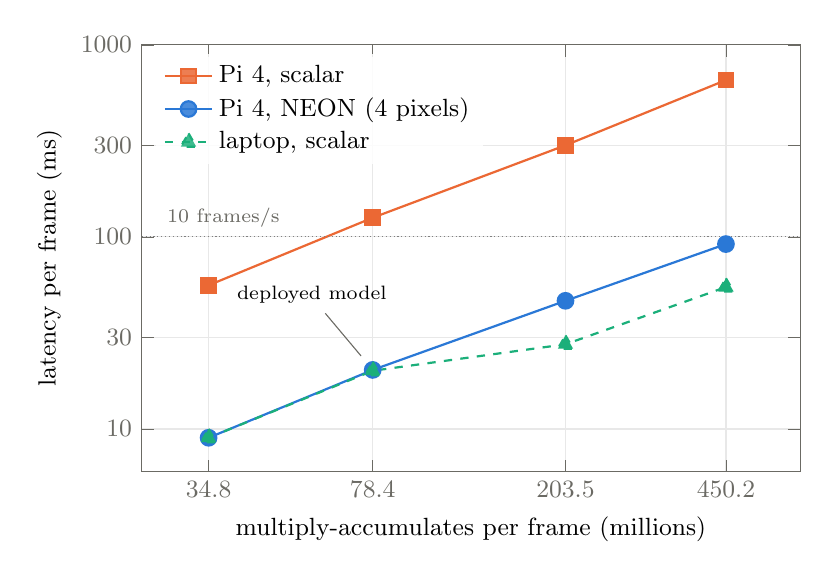
\begin{tikzpicture}
\begin{loglogaxis}[
  width=0.82\textwidth, height=7cm,
  xlabel={multiply-accumulates per frame (millions)},
  ylabel={latency per frame (ms)},
  xmin=25, xmax=650, ymin=6, ymax=1000,
  xtick={34.8,78.4,203.5,450.2}, xticklabels={34.8,78.4,203.5,450.2},
  ytick={10,30,100,300,1000}, yticklabels={10,30,100,300,1000},
  axis line style={inkmuted}, tick style={inkmuted},
  ticklabel style={font=\small, text=inkmuted}, label style={font=\small},
  grid=major, major grid style={gray!18},
  legend style={at={(0.02,0.98)}, anchor=north west, font=\small, draw=none, fill=white, fill opacity=0.85, text opacity=1},
  legend cell align=left,
]
\addplot[s2, thick, mark=square*, mark size=2.6pt] coordinates {(34.8,56.0) (78.4,125.9) (203.5,300.1) (450.2,656.0)};
\addlegendentry{Pi 4, scalar}
\addplot[s1, thick, mark=*, mark size=2.8pt] coordinates {(34.8,9.0) (78.4,20.3) (203.5,46.5) (450.2,91.8)};
\addlegendentry{Pi 4, NEON (4 pixels)}
\addplot[s3, thick, dashed, mark=triangle*, mark size=3.2pt] coordinates {(34.8,9.0) (78.4,20.1) (203.5,27.6) (450.2,54.8)};
\addlegendentry{laptop, scalar}
\addplot[gray, densely dotted] coordinates {(25,100) (650,100)};
\node[font=\scriptsize, text=inkmuted, anchor=south west] at (axis cs:27,100) {10 frames/s};
\draw[inkmuted] (axis cs:74,24) -- (axis cs:62,40);
\node[font=\scriptsize, anchor=south] at (axis cs:58,40) {deployed model};
\end{loglogaxis}
\end{tikzpicture}
\caption{Latency against compute, one core, logarithmic axes (the four
models of Table~\ref{tab:latency}). Slope 1 means constant GMAC/s. The two
leftmost Pi NEON points coincide with the laptop's scalar points.}
\label{fig:latency}
\end{figure}

\subsection{Four cores, temperature and memory}

\begin{table}[H]
\centering
\caption{Four independent copies in parallel (one frame per copy at a
time), four-pixel NEON kernel; per-copy latency range, total frames per
second, temperature at the end of a 1--3 minute run, and peak resident
memory of one process.}
\label{tab:fourcore}
\begin{tabular}{lrrrrr}
\toprule
Model & 1 core, ms & Per copy, ms & Frames/s & End temp. & Peak memory \\
\midrule
\cfg{small} $240{\times}160$ & 9.0 & 9.3--9.4 & 425 & \SI{58.9}{\celsius} & 1.8 MB \\
\textbf{\cfg{small} $360{\times}240$} & 20.3 & 21.0--21.3 & \textbf{187} & \SI{64.2}{\celsius} & \textbf{2.3 MB} \\
\cfg{small\_wide} $360{\times}240$ & 46.5 & 59.1--59.5 & 67.1 & \SI{72.0}{\celsius} & 2.6 MB \\
\cfg{wide} $480{\times}320$ & 91.8 & 100.5--101.5 & 39.4 & \SI{78.8}{\celsius} & 3.4 MB \\
\bottomrule
\end{tabular}
\end{table}

The 32-channel models scale 3.8 times on four cores; the 64-channel models
3.1--3.6 times (with the single-pixel kernel only 1.9--2.2 times). The
four-copy scalar run of \cfg{wide}, the heaviest load, reached
\SI{81.8}{\celsius} and set the firmware's soft-temperature-limit flag
(\texttt{0x80000}), with a 1\,\% effect on latency; the flag stays set
until reboot, so later runs could not be checked for throttling by it, but
all stayed below \SI{80}{\celsius}. For the deployed model the program
file is 54~KB, of which 42~KB are weights; the static buffers are 854~KB
(two 355~KB activation buffers, the head map, and the 83~KB 16-bit weight
copy).

\subsection{MCNN under the same protocol: accuracy}
\label{sec:mcnnacc}

\begin{table}[H]
\centering
\caption{Naming the 2\,826 annotated objects, five-fold scene CV, mean
$\pm$ s.d.\ over three seeds. ``Missed'': no detection overlaps the box.}
\label{tab:mcnnacc}
\resizebox{\textwidth}{!}{%
\begin{tabular}{lcccccccccc}
\toprule
Model & Params & Boxes given & Accuracy (\%) & Macro-F1 (\%) & Missed (\%) & \multicolumn{5}{c}{Accuracy per fold (\%)} \\
\cmidrule(lr){7-11}
 & & & & & & 0 & 1 & 2 & 3 & 4 \\
\midrule
MCNN                    & \num{2797706} & yes & $77.7 \pm 0.5$ & $71.4 \pm 1.7$ & --  & 84.5 & 89.6 & 47.0 & 83.6 & 78.5 \\
\cfg{small} $360{\times}240$       & \num{42463} & no  & $74.2 \pm 1.3$ & $70.4 \pm 3.0$ & 7.4 & 83.8 & 85.1 & 55.4 & 62.1 & 70.8 \\
\cfg{small\_wide} $360{\times}240$ & \num{135359} & no  & $77.6 \pm 2.4$ & $74.4 \pm 2.7$ & 6.3 & 85.7 & 88.8 & 63.0 & 68.7 & 70.3 \\
\bottomrule
\end{tabular}}
\end{table}

\begin{figure}[H]
\centering
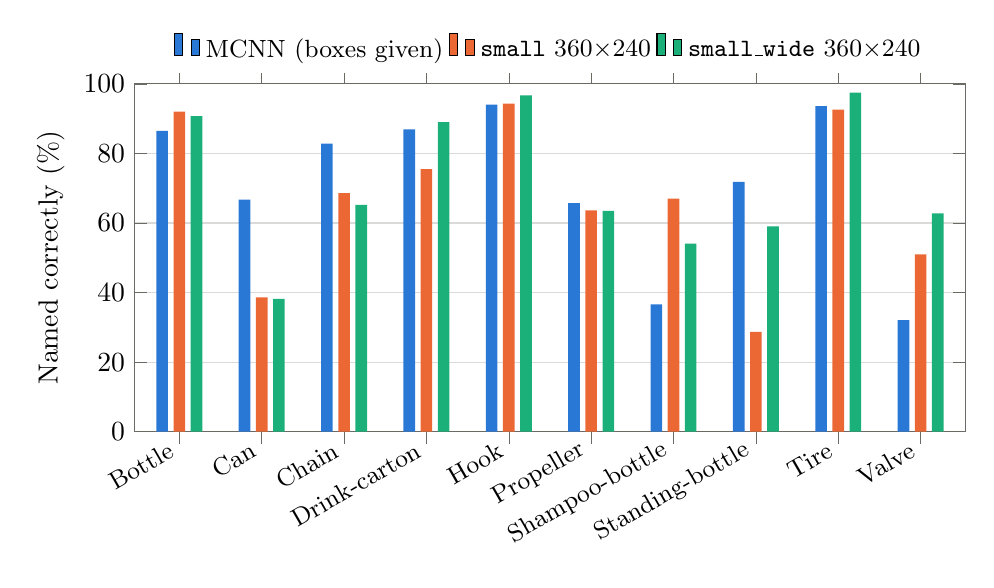
\begin{tikzpicture}
\begin{axis}[
  ybar, bar width=4.2pt, width=\textwidth, height=6cm,
  ymin=0, ymax=100, ylabel={Named correctly (\%)},
  symbolic x coords={Bottle,Can,Chain,Drink-carton,Hook,Propeller,Shampoo-bottle,Standing-bottle,Tire,Valve},
  xtick=data, x tick label style={rotate=30, anchor=east, font=\small},
  ymajorgrids, grid style={inkmuted!25}, axis line style={inkmuted}, tick style={inkmuted},
  legend style={at={(0.5,1.03)}, anchor=south, legend columns=3, draw=none, font=\small},
  enlarge x limits=0.06,
]
\addplot[fill=s1, draw=none] coordinates {(Bottle,86.5) (Can,66.7) (Chain,82.8) (Drink-carton,86.9) (Hook,94.0) (Propeller,65.7) (Shampoo-bottle,36.6) (Standing-bottle,71.8) (Tire,93.6) (Valve,32.1)};
\addplot[fill=s2, draw=none] coordinates {(Bottle,92.0) (Can,38.6) (Chain,68.6) (Drink-carton,75.5) (Hook,94.3) (Propeller,63.6) (Shampoo-bottle,67.0) (Standing-bottle,28.7) (Tire,92.6) (Valve,51.0)};
\addplot[fill=s3, draw=none] coordinates {(Bottle,90.7) (Can,38.2) (Chain,65.2) (Drink-carton,89.0) (Hook,96.7) (Propeller,63.5) (Shampoo-bottle,54.1) (Standing-bottle,59.0) (Tire,97.5) (Valve,62.8)};
\legend{MCNN (boxes given), \cfg{small} $360{\times}240$, \cfg{small\_wide} $360{\times}240$}
\end{axis}
\end{tikzpicture}
\caption{Per-class recall on the naming task, mean of three seeds, pooled
over the five folds.}
\label{fig:recall}
\end{figure}

\subsection{MCNN under the same protocol: speed and memory}
\label{sec:mcnnspeed}

\begin{table}[H]
\centering
\caption{Raspberry Pi~4. ONNX Runtime 1.31.1, float32, same engine for all
models; repeats agree within 1.5\,\%. Peak memory includes the 45.5~MB of
the interpreter with ONNX Runtime loaded. C int8: this project's runtime,
NEON, one thread.}
\label{tab:mcnnspeed}
\resizebox{\textwidth}{!}{%
\begin{tabular}{lrrlrrrr}
\toprule
Model & Params & MMAC & Unit & ORT 1 thread, ms & ORT 4 threads, ms & C int8, ms & Peak memory ORT / C \\
\midrule
MCNN       & \num{2797706} & 234.7 & per crop  & 66.5  & 24.7 & --   & 75.5 MB / -- \\
           &               & 355   & per frame (1.51 crops) & 100.6 & 37.4 & --   &  \\
\cfg{small} $360{\times}240$       & \num{42463}  & 78.4  & per frame & 22.4 & 8.8  & 20.3 & 58.1 MB / 2.3 MB \\
\cfg{small\_wide} $360{\times}240$ & \num{135359} & 203.5 & per frame & 48.7 & 17.2 & 46.5 & 58.7 MB / 2.6 MB \\
\bottomrule
\end{tabular}}
\end{table}

The ONNX model files are 11.2~MB (MCNN), 0.17~MB (\cfg{small}) and
0.54~MB (\cfg{small\_wide}). Note that the ONNX Runtime four-thread figures
are one frame spread over four cores, unlike the four-copy throughput of
Table~\ref{tab:fourcore}.

\subsection{Segmentation head}

\begin{table}[H]
\centering
\small
\caption{Segmentation head on \cfg{small} $360 \times 240$, five-fold CV.
mIoU over 12 labels. Ceiling of the cell-centre labelling itself: 77.2 mIoU
at stride 8, 87.0 at stride 4 (development test fold).}
\label{tab:seg}
\begin{tabular}{lrrr}
\toprule
Variant & Extra MACs & Pooled mIoU & Pooled box mAP \\
\midrule
Boxes only (3 seeds) & -- & -- & 52.6 (1.9) \\
Stride 8, weighted cross-entropy & 0.3 M & 33.9 & 52.1 \\
Stride 4 (sub-pixel) & 1.6 M & 35.0 & 52.0 \\
Stride 4 + Dice, weight 1 (2 seeds) & 1.6 M & 42.0 (1.1) & 50.3 (0.7) \\
Stride 4 + Dice, weight 0.3 & 1.6 M & 38.9 & 51.1 \\
\cfg{small\_wide} backbone, stride 4 + Dice & 1.6 M & 46.2 & 56.3 \\
\bottomrule
\end{tabular}
\end{table}

The int8 masks equal the float masks (33.8 against 33.9 mIoU), and the C
runtime emits the label map, checked cell by cell by the golden test.

\subsection{Independence of the folds}
\label{sec:independence}

For every frame, the most similar frame in a \emph{different} fold was found
by correlation of $32 \times 48$ mean-centred, normalised thumbnails.

\begin{table}[H]
\centering
\caption{Nearest frame in another fold (thumbnail correlation).}
\label{tab:indep}
\begin{tabular}{lcc}
\toprule
Split & Median correlation & Frames with a match $> 0.95$ \\
\midrule
Random frame-level 5-fold & 0.998 & 99.8\,\% \\
Scene 5-fold (this work) & 0.966 & 62.3\,\% \\
\midrule
\multicolumn{3}{l}{\emph{Reference values}} \\
Nearest frame in the same scene & 0.998 & -- \\
Random pair of frames & 0.747 & -- \\
\bottomrule
\end{tabular}
\end{table}

In addition, the 1\,868 frames contain 43 distinct combinations of object
classes (ignoring position); 22 of them occur in more than one fold.

% ===========================================================================
\section{Discussion}

\subsection{Evaluation protocol}

The scene folds remove the near-copies that random splits place across the
boundary: under a random split the nearest frame in another fold is as
similar (0.998) as the nearest frame of the same recording, i.e.\ the test
set is the training set seen again. Under the scene folds the figure drops
to 0.966. It does not fall to the level of unrelated frames (0.747), and 22
of the 43 object combinations span several folds: the same objects, moved or
seen from a different angle, can be in training and test. The linking rule
was deliberately conservative toward the training set (it links only
frames whose boxes coincide), so the residual dependence is in this
direction, and the reported figures may still be optimistic. Part of the
remaining similarity is the shared tank background, which every frame has.
A stricter grouping by object combination is the next test
(Section~\ref{sec:further}).

The price of the scene folds is large fold-to-fold variation (per-fold mAP
42--73), which is a property of the data: classes concentrated in one scene
cannot be both trained and tested well under any split. The relevant noise
figure for comparing configurations is the seed spread of the pooled mAP
(1--3 points), not the per-fold spread. Development-split values are 10--15
points above the pooled values because fold 0 is easy.

\subsection{Resolution and width}

The \cfg{wide} model's lead over \cfg{small} at $240 \times 160$ (+7 pooled)
is mostly input resolution: the unchanged \cfg{small} network at
$360 \times 240$ gains 4.5 points on three-seed means (every seed pairing,
every fold), and saturates there ($480 \times 320$: 54.1). The gains are in
the small objects (bottle, can, chain, valve), whose extent at half
resolution approaches the 8-pixel stride. Width alone does nothing at
$240 \times 160$ (\cfg{small\_wide} +0.8, within noise) but adds 4.3 points
at $360 \times 240$ (56.9 $\pm$ 2.7 against 52.6 $\pm$ 1.9, above the
deployed model on every seed and fold mean), matching \cfg{wide} at 45\,\%
of its compute. The interpolation does not hold: 48 channels give no gain
(50.9). The 64-channel model's largest and least stable gain is
standing-bottle (23.7 $\pm$ 14.0), a single-scene class.

\subsection{Quantisation and the runtime}

Post-training int8 quantisation is free within seed noise for every
configuration, and the C runtime is bit-exact with the integer reference on
x86 and ARM, with and without the NEON kernel. The practical consequence is
that cross-validated accuracy transfers to the device by construction; the
30-model on-device CV (Table~\ref{tab:ondevice}) confirms it empirically.

On the Pi the scalar runtime is limited by what the compiler makes of the
inner loop (0.6--0.7 GMAC/s); the hand-written NEON kernel gives 6.2--7.1
times that. The four-pixel version's pattern of gains (11--13\,\% for
32-channel models whose 16-bit weights fit the 32~KB L1 cache, 1.5--1.7
times for 64-channel models whose 74~KB weight tables do not, and much better
four-core scaling) supports weight traffic as the limit of the single-pixel
kernel. Cache misses were not counted directly.

The same-engine comparison shows that the speed of the deployed system comes
mainly from the network's size, not from the runtime: ONNX Runtime in float
runs \cfg{small} in 22.4~ms against 20.3~ms for the int8 C runtime. The
runtime's contributions are memory (2.3~MB against 58~MB), the absence of
any dependency, a 42~KB weight file, and exactness across platforms.

\subsection{Detector against MCNN}

Under the scene folds MCNN reaches 77.7\,\%, not 99.8\,\%: most of the
published accuracy is the leak of the random split. On MCNN's own task, and
without being given the boxes, \cfg{small\_wide} matches its accuracy
(77.6) and exceeds its macro-F1 (74.4 against 71.4), with 20 times fewer
parameters; the deployed \cfg{small} is 3.5 points lower in accuracy with 66
times fewer. The F1 difference is about one seed standard deviation, so the
firm statement is ``on a par'', not ``better''. Among the objects the
detectors do find (92--94\,\%), they name more correctly than MCNN.

The per-class pattern has two explanations. MCNN sees the box outline, and
with it the object's size and aspect ratio, which alone predict the class
almost perfectly on the random split (Table~\ref{tab:predecessor}); its
advantage is concentrated in fold~3 (the tall, narrow standing bottles:
83.6 against 62--69). Conversely, fold 2 holds two thirds of the valves, so
its models train on 69; MCNN names 17\,\% of the fold-2 valves and the
detectors, which see the objects' surroundings, degrade less.

In cost, the deployed detector processes a whole frame 4.5 times faster
than MCNN classifies the objects in it (22.4 against 100.6~ms in the same
engine; 78 against 355~M MACs), and MCNN additionally needs a stage that
finds the objects, which the paper does not specify.

\subsection{Choice of the deployed model}

Two operating points are available:

\begin{center}
\resizebox{\textwidth}{!}{%
\begin{tabular}{lcccccc}
\toprule
 & mAP on Pi & Naming acc. & ms / frame & Frames/s & Memory & Params \\
\midrule
\cfg{small} $360{\times}240$ & 52.3 & 74.2\,\% & 20.3 & 49 & 2.3 MB & \num{42463} \\
\cfg{small\_wide} $360{\times}240$ & 56.7 & 77.6\,\% & 46.5 & 21.5 & 2.6 MB & \num{135359} \\
\bottomrule
\end{tabular}}
\end{center}

Both exceed the frame rate of the sonar (an ARIS records on the order of
10--15 frames/s depending on range, to be confirmed for these recordings),
so either keeps up in real time on one core; \cfg{small\_wide}'s extra cost
appears as energy and heat rather than dropped frames.

% ===========================================================================
\section{Sources of error and limitations}

\begin{itemize}
  \item \textbf{Residual dependence across folds} (Section~\ref{sec:independence}):
        the same objects can appear in several folds; reported accuracies may
        be optimistic.
  \item \textbf{Single-scene classes}: standing-bottle is testable only by a
        model trained on four instances; its AP measures the dataset.
        Valve and drink-carton are similar to a lesser degree.
  \item \textbf{Seed variation}: three seeds for the main configurations,
        one for the others; differences under about 3 points are not
        resolved.
  \item \textbf{Water tank only}: no frames from open water were evaluated;
        generalisation to field conditions is untested.
  \item \textbf{Scope of ``end-to-end''}: timing starts from the Cartesian
        image in memory. The projection from raw polar sonar data and the
        resize to $360 \times 240$ (done in Python) are not included.
  \item \textbf{Throughput}: the four-core figures are independent copies;
        the runtime has no multi-threaded single-frame mode.
  \item \textbf{Thermal}: runs lasted 1--3 minutes without a fan; steady
        state under sustained load was not measured.
  \item \textbf{Energy}: not measured.
  \item \textbf{MCNN comparison}: MCNN is given the true boxes and uses the
        reimplementation's recipe (30 epochs, no augmentation); it was timed
        in floating point only. An int8 MCNN or an int8 ONNX detector was not
        built.
  \item \textbf{Wall} is scored like the other classes although its boxes
        are large and loosely defined.
\end{itemize}

% ===========================================================================
\section{Conclusions}

\begin{enumerate}
  \item A scene-grouped, class-balanced five-fold protocol is in place; it
        removes the near-copy leak of random splits (nearest cross-fold
        frame 0.966 instead of 0.998) but not all dependence between folds.
  \item The deployed detector (\cfg{small}, $360 \times 240$, 42~k
        parameters, 78~M MACs) reaches \textbf{52.3 $\pm$ 1.7 mAP@0.5
        measured on the Raspberry Pi~4}; \cfg{small\_wide} reaches
        \textbf{56.7 $\pm$ 2.7} at 2.6 times the compute.
  \item Input resolution is the main lever, saturating at
        $360 \times 240$; 64-channel width pays only at that resolution.
  \item Post-training int8 quantisation costs nothing measurable; the C
        runtime is bit-exact with the reference on x86 and ARM, so the
        accuracy holds on the device by construction and was confirmed on 30
        models.
  \item With a NEON kernel exact by construction, the deployed model runs
        in \textbf{20.3~ms per frame on one Cortex-A72 core} (49 frames/s;
        187 frames/s with four independent copies) in \textbf{2.3~MB}.
  \item Under the same protocol MCNN reaches 77.7\,\% (99.8\,\% on the
        random split). Without the boxes, \cfg{small\_wide} names the objects
        as accurately (77.6\,\%, macro-F1 74.4 against 71.4) with 20 times
        fewer parameters, and the deployed detector processes a frame 4.5
        times faster than MCNN classifies its objects.
\end{enumerate}

% ===========================================================================
\section{Further work}
\label{sec:further}

\begin{enumerate}
  \item \textbf{Stricter grouping}: group frames by object combination
        (about 43 groups), stratified group $K$-fold with $K = 3$ or 5 and
        validation scenes drawn from the training part; rerun detectors and
        MCNN.
  \item \textbf{Paper protocol for both}: train the detectors on a random
        90/10 split as MCNN was, to show the inflation symmetrically; paired
        test of the F1 difference over the 15 fold--seed pairs.
  \item \textbf{Front end}: a lookup-table remap in C from raw polar beam
        data directly to the $360 \times 240$ input, timed on the Pi.
  \item \textbf{Single-frame multi-core}: split each layer's rows across
        four threads (bit-exact) to report per-frame latency on four cores.
  \item \textbf{Sustained thermal run}: 30 minutes at both operating
        points, logging temperature, clock and latency.
  \item \textbf{Energy}: inline USB-C meter or INA219/INA226 sensor;
        energy per frame from loaded minus idle power.
  \item \textbf{Raspberry Pi~5}: the same program, plus a kernel using the
        8-bit dot-product instructions; the Pi~5's power-management chip
        also reports rail currents.
  \item \textbf{External data}: a qualitative run on the 7\,200 unlabelled
        real-water quarry frames of the same collection, then hand-labelling a
        subset as an independent test set.
  \item \textbf{Accuracy}: knowledge distillation from \cfg{wide};
        class-balanced sampling and copy--paste augmentation for can,
        standing-bottle and valve.
\end{enumerate}

% ===========================================================================
\begin{thebibliography}{9}\raggedright
\bibitem{cimen} \c{C}imen and Bolat, ``MCNN: A customized CNN model for marine debris classification based on sonar images.''
\bibitem{valdenegro2025} M.~Valdenegro-Toro, D.~C.~Padmanabhan, D.~Singh, B.~Wehbe and Y.~Petillot,
  \emph{The marine debris forward-looking sonar datasets}, arXiv:2503.22880, 2025.
  Repository \texttt{mvaldenegro/marine-debris-fls-datasets}, commit \texttt{4a77998}.
\bibitem{zhou2019} X.~Zhou, D.~Wang and P.~Kr\"ahenb\"uhl, ``Objects as points,'' arXiv:1904.07850, 2019.
\bibitem{law2018} H.~Law and J.~Deng, ``CornerNet: Detecting objects as paired keypoints,'' in \emph{ECCV}, 2018.
\bibitem{jacob2018} B.~Jacob et al., ``Quantization and training of neural networks for efficient integer-arithmetic-only inference,'' in \emph{CVPR}, 2018.
\end{thebibliography}

% ===========================================================================
\appendix
\section{Reproduction}
\label{app:repro}

\begin{small}
\begin{verbatim}
# scene groups and folds (writes splits/scene_folds_v1.json)
uv run python -m sonar_edge.split
# 5-fold CV of one configuration and seed; pool; aggregate seeds
./run_cv.sh small_360_cv small 4/3 150 strong 0  # -> runs/small_360_cv_f{0..4}
uv run sonar-edge cv runs/small_360_cv
uv run sonar-edge seeds runs/small_360_cv runs/small_360_s1_cv runs/small_360_s2_cv
# quantise, export to C, test, score the C runtime
uv run sonar-edge quantize runs/<run>/best.pt
uv run python -m sonar_edge.export_c runs/<run>
make -C runtime test
uv run python -m sonar_edge.c_eval runs/<run>
# score detections produced on the Pi (per fold), then pool with variant pi4
uv run python -m sonar_edge.c_eval runs/<run> --test-fold k --val-fold k+1 \
    --pred dets.txt --tag pi4
# MCNN on the scene folds; detector on MCNN's task
uv run python -m sonar_edge.mcnn_cv train --seeds 0 1 2
uv run python -m sonar_edge.mcnn_cv summary
uv run python -m sonar_edge.gt_cls runs/small_360_cv runs/small_360_s1_cv \
    runs/small_360_s2_cv --variant pi4
\end{verbatim}
\end{small}

\section{Milestone documents}

The repository's \texttt{docs/} folder holds one technical note per
milestone with the full derivations: M0 data and protocol, M1 detector and
ablations, M2 quantisation, M3 runtime, M4 pipeline verification, M5 Pi
benchmark and NEON kernel, M6 segmentation, M7 on-device CV and MCNN
comparison. Earlier reports: \texttt{report/overview.pdf} (data, model,
runtime), \texttt{report/deployment.pdf} (Pi measurements),
\texttt{report/comparison.pdf} (on-device CV, MCNN comparison).

\end{document}
